%  This is a LaTex file.

%  Homework for the course "AMath 585:  Applied Linear Algebra and Numerical Analysis",
%  Autumn quarter, 2009, Anne Greenbaum.


%   A latex format for making homework assignments.


\documentclass[letterpaper,12pt]{article}

%          The page format, somewhat wider and taller page than in art12.sty.

\topmargin -0.1in \headsep 0in \textheight 8.9in \footskip 0.6in
\oddsidemargin 0in  \evensidemargin 0in  \textwidth 6.5in
\usepackage{graphicx}
\usepackage{listings}
\usepackage{caption}
\usepackage{subcaption}
\usepackage{color}
\usepackage{float}
\definecolor{keywords}{RGB}{255,0,90}
\definecolor{comments}{RGB}{0,0,113}
\definecolor{red}{RGB}{160,0,0}
\definecolor{green}{RGB}{0,150,0}
\definecolor{codegreen}{rgb}{0,0.6,0}
\definecolor{codegray}{rgb}{0.5,0.5,0.5}
\definecolor{codepurple}{rgb}{0.58,0,0.82}
\definecolor{backcolour}{rgb}{0.95,0.95,0.92}
\definecolor{brown}{rgb}{0.59, 0.29, 0.0}
\definecolor{beaublue}{rgb}{0.74, 0.83, 0.9}
\definecolor{orange}{rgb}{1.0, 0.5, 0.0}
\definecolor{darkslategray}{rgb}{0.18, 0.31, 0.31}
\definecolor{deepblue}{rgb}{0,0,0.5}
\definecolor{deepred}{rgb}{0.6,0,0}
\definecolor{deepgreen}{rgb}{0,0.5,0}
\lstdefinestyle{myMatlabstyle}{
	language=Matlab,
	backgroundcolor=\color{white},
	commentstyle=\color{codegreen},
	keywordstyle=\color{blue},
	%identifierstyle=\color{brown},
	numberstyle=\tiny\color{codegray},
	stringstyle=\color{orange},
	basicstyle=\footnotesize,
	breakatwhitespace=false,
	breaklines=true,
	captionpos=b,
	keepspaces=true,
	numbers=left,
	numbersep=5pt,
	showspaces=false,
	showstringspaces=false,
	showtabs=false,
	tabsize=2
}
\lstdefinestyle{myPythonstyle}{
	language=Python,
	basicstyle=\ttfamily\small,
	keywordstyle=\color{blue},
	backgroundcolor=\color{white},
	commentstyle=\color{green},
	stringstyle=\color{red},
	showstringspaces=false,
	%identifierstyle=\color{brown},
	breaklines=true,
}
\lstset{language=Matlab,frame=single}
\lstset{language=Python,frame=single}
\usepackage{amsmath}
\usepackage{epsfig}         % to insert PostScript figures
       % to insert PostScript figures

\begin{document}


%          Definitions of commonly used symbols.



%          The title and header.

\noindent
{\scriptsize ES$\_$APPM 420-1, Fall 2018} \hfill

\begin{center}
\large
Assignment 1.
\normalsize

Jithin D. George
\end{center}

\noindent
Due Oct 17

\vspace{.3in}

%           The questions!



\noindent


\begin{enumerate}
\item
\[x^2 +(1-\epsilon - \epsilon^2)x+\epsilon-2e^{\epsilon^2}=0\]
Let us assume
\[x = x_0 + x_1\epsilon^{r}+ x_2\epsilon^{2r} + x_3\epsilon^{3r} +\hdots\]
\[x^2 = x_0^2 + 2 x_0 x_1\epsilon^{r}+ 2(x_0x_2+x_1^2)\epsilon^{2r}  +\hdots\]
Plugging this into the algebraic equation,
\begin{align*}
x_0^2 + 2 x_0 x_1\epsilon^{r}+ 2(x_0x_2+x_1^2)\epsilon^{2r}  +x_0 + x_1\epsilon^{r}+ x_2\epsilon^{2r} - x_0 \epsilon - x_1\epsilon^{1+r}- x_2\epsilon^{1+2r} \\
- x_0 \epsilon^2 - x_1\epsilon^{2+r}- x_2\epsilon^{2+2r} + \epsilon - 2 -2\epsilon^2-\epsilon^4 +\hdots =0
\end{align*}
Equating the zero order terms,
\[x_0^2+x_0-2=0\]
\[x_0 = -2,1\]
For dominant balance, we need
\[\epsilon^r \approx \epsilon\]
\[r=1\]
Equating the zero order terms,
\[x_0^2+x_0-2=0\]
\[x_0 = -2,1\]
Equating the first order terms,
\[2x_0x_1+x_1-x_0+1=0\]
\[x_1 = 1,0\]
Equating the second  order terms,
\[2x_0x_2+2x_1^2+x_2-x_1-x_0-2=0\]
\[x_2 = 0.5,1\]
So, the solutions are
\[x = -2 + \epsilon+ \frac{1}{2}\epsilon^{2}  +O(\epsilon^3)\]
and
\[x = 1 +  \epsilon^{2}  +O(\epsilon^3)\]

\item
\[\epsilon x^3 - 3x+1=0\]
Let us assume
\[x = \delta_0 x_0 + x_1 \delta_1+ x_2 \delta_2 + x_3 \delta_3 +\hdots\]
\[x^3 = \delta_0^3 x_0^3 + 3 \delta_0^2 \delta_1 x_0^2 x_1   + 3 \delta_0^2 \delta_2 x_0^2 x_2 +3 \delta_1^2 \delta_0 x_1^2 x_0   +   \hdots\]

Trying the dominant terms,
\[\epsilon \delta_0^3 x_0^3- 3 \delta_0 x_0 +1 =0 \]
Dominant balance gives two options
\[ \delta_0 \sim 1, \delta_0 \sim \epsilon^{-\frac{1}{2}}\]
And
\[x_0 = \frac{1}{3},x_0^3-3x_0=0 \to x_0 = \sqrt{3}, -\sqrt{3}\]

Equating the next  order terms,
\[3 \delta_0^2 \delta_1 x_0^2 x_1 \epsilon - 3x_1 \delta_1 =0\]
\[x_0 = -2,1\]

Let $x = r \epsilon^{-\frac{1}{2}}$. Then the main equation becomes

\[\frac{r^3}{\sqrt{\epsilon}}- 3\frac{r}{\sqrt{\epsilon}}+1=0\]
\[r^3-3r+\sqrt{\epsilon}=0\]

\[r = r_0 + r_1\epsilon^{a}+ r_2\epsilon^{2a} + r_3\epsilon^{3a} +\hdots\]
\[r^3 = r_0^3 + 3 r_0^2 r_1\epsilon^{a}+ 3(r_0r_2+r_1^2)\epsilon^{2a}  +\hdots\]

\[r_0^3 + 3 r_0^2 r_1\epsilon^{a}+ 3(r_0r_2+r_1^2)\epsilon^{2a} -3 r_0 -3 r_1\epsilon^{a}-3 r_2\epsilon^{2a} -3 r_3\epsilon^{3a} + \sqrt{\epsilon}=0\]

Equating the zero order terms,
\[r_0^3-3r_0=0\]
\[r_0 = 0,-\sqrt{3},\sqrt{3}\]
Equating the next order terms,
\[a = \frac{1}{2}\]
\[3 r_0^2 r_1 -3 r_1 + 1=0\]
\[r_1 = \frac{1}{3},\frac{1}{6},\frac{1}{6}\]
Equating the next order terms,
\[3(r_0r_2+r_1^2)-3r_2=0\]
\[r_2 = \frac{1}{9},...\]
So, the solutions in r  are
\[r =   \frac{1}{3}\epsilon^{\frac{1}{2}}+ \frac{1}{9}\epsilon  +O(\epsilon^3)\]
\[r = -\sqrt{3} + \frac{1}{6}\epsilon^{\frac{1}{2}}+  +O(\epsilon)\]
\[r = \sqrt{3} +  \frac{1}{6}\epsilon^{\frac{1}{2}}+ +O(\epsilon^)\]
and thus,
\[x =   \frac{1}{3}+ \frac{1}{9}\epsilon^{\frac{1}{2}} +O(\epsilon)\]
\[x = -\sqrt{3}\epsilon^{-\frac{1}{2}} + \frac{1}{6}  +O(\epsilon^{\frac{1}{2}})\]
\[x = \sqrt{3}\epsilon^{-\frac{1}{2}} +  \frac{1}{6} +O(\epsilon^{\frac{1}{2}})\]
\item
\[\epsilon^2x^3-x+\epsilon=0\]
Trying dominant balance,
\[\epsilon^2\delta_0^3x_0^3-x_0\delta_0+\epsilon=0\]
There are two options.
\[\delta_0 \sim \epsilon, \delta_0 \sim \epsilon^{-1}\]

The second option is the more 'dominant' of the two. So, we can rescale the original equation by it.

 Let
 \[x = r\epsilon^{-1}\]
 \[r^3-r+\epsilon^2=0\]

 \[r = r_0 + r_1\epsilon^{a}+ r_2\epsilon^{2a} + r_3\epsilon^{3a} +\hdots\]
 \[r^3 = r_0^3 + 3r_0^2 r_1\epsilon^{a}+ 3(r_0r_2+r_1^2)\epsilon^{2a}  +\hdots\]

\[ r_0^3 + 3r_0^2 r_1\epsilon^{a}+ 3(r_0r_2+r_1^2)\epsilon^{2a}- r_0 - r_1\epsilon^{a}- r_2\epsilon^{2a} - r_3\epsilon^{3a} +\epsilon^2 +\hdots= 0\]
Equating the zero order terms,
\[r_0^3-r_0=0\]
\[r_0 = 0,-1,1\]
Equating the next order terms,
\[a = 2\]
\[3 r_0^2 r_1 - r_1 + 1=0\]
\[r_1 = 1,-\frac{1}{2},-\frac{1}{2}\]
Equating the next order terms,
\[3(r_0r_2+r_1^2)-r_2=0\]
\[r_2 = 1,...\]
So, the solutions in r  are
\[r =  \epsilon^{2}+ \epsilon^4  +O(\epsilon^6)\]
\[r = -1- \frac{1}{2}\epsilon^{2}+  +O(\epsilon^4)\]
\[r = 1 -  \frac{1}{2}\epsilon^{2}+ +O(\epsilon^4)\]
and thus,
\[x =   \epsilon+ \epsilon^3  +O(\epsilon^5)\]
\[x = -\frac{1}{\epsilon}- \frac{1}{2}\epsilon+  +O(\epsilon^3)\]
\[x = \frac{1}{\epsilon}- \frac{1}{2}\epsilon+  +O(\epsilon^3)\]

\item
\[x^2 + \sqrt{1+ \epsilon x} = e^{\frac{1}{2+\epsilon}}\]

This is not singular. So,

\[x = x_0 + x_1\epsilon^{r}+ x_2\epsilon^{2r} + x_3\epsilon^{3r} +\hdots\]

\[x_0^2+ 2 x_0 x_1 \epsilon^r + \sqrt{1+ \epsilon x_0 + x_1\epsilon^{r+1} +\hdots} = e^{\frac{1}{2+\epsilon}}+ \hdots \]
\[x_0^2+ 2 x_0 x_1 \epsilon^r + 1+  \frac{1}{2} \epsilon  x_0 +\frac{1}{2} x_1\epsilon^{r+1}  = e^{\frac{1}{2+\epsilon}} = \sqrt{e}-\sqrt{e}\frac{\epsilon}{4}\]
From here, it is clear that
\[r = 1\]
\[x_0 = \sqrt{\sqrt{e}-1},- \sqrt{\sqrt{e}-1}\]
\[x_1 =- \frac{\sqrt{e}}{4\sqrt{\sqrt{e}-1}} - \frac{1}{4}, \frac{\sqrt{e}}{4\sqrt{\sqrt{e}-1}} - \frac{1}{4}\]

So, the solutions are
\[x = \sqrt{\sqrt{e}-1} - \frac{\sqrt{e}}{4\sqrt{\sqrt{e}-1}}\epsilon - \frac{1}{4}\epsilon + o(\epsilon )\]
and
\[x = -\sqrt{\sqrt{e}-1} + \frac{\sqrt{e}}{4\sqrt{\sqrt{e}-1}}\epsilon - \frac{1}{4}\epsilon + o(\epsilon )\]
\item
\[x^2 + \epsilon\sqrt{2+x}= cos(\epsilon)\]

\[x = x_0 + x_1\epsilon^{r}+ x_2\epsilon^{2r} + x_3\epsilon^{3r} +\hdots\]

\[x_0^2+ 2 x_0 x_1 \epsilon^r + \epsilon \sqrt{2+ x_0 + x_1\epsilon^{r}+\hdots}=1-\frac{\epsilon^2}{2}+\hdots\]

\[x_0^2+ 2 x_0 x_1 \epsilon^r + \epsilon \sqrt{2+ x_0} +\frac{ x_1\epsilon^{r+1}}{2\sqrt{2+ x_0}} +\hdots=1-\frac{\epsilon^2}{2}+\hdots \]

From here, it is clear that
\[r = 1\]
\[x_0 = 1,-1\]
\[x_1 = - \frac{3}{2}, \frac{1}{2}\]

Thus, the solutions are

\[x =1 - \frac{3}{2}\epsilon +o(\epsilon)\]
\[x =-1 + \frac{1}{2}\epsilon +o(\epsilon)\]
\item
\[ \epsilon e^{x^2}= 1 + \frac{\epsilon}{1+x^2}\]
\[ \epsilon e^{x^2}+ x^2 \epsilon e^{x^2}= 1+ x^2 + \epsilon\]
Using  the dominant terms,
\[ \epsilon e^{x_0^2 \delta_0^2}+ x_0^2\delta_0^2 \epsilon e^{x_0^2\delta_0^2}= 1+ x_0^2\delta_0^2 + \epsilon\]
The dominant balance seems to be
\[ \delta_0^2 \epsilon e^{\delta_0^2} \sim \delta_0^2 \]
\[ e^{\delta_0^2} \sim \frac{1}{\epsilon}\]
\[ \delta_0 \sim \sqrt{\log \frac{1}{\epsilon}}\]
Let
\[x = r  \sqrt{\log \frac{1}{\epsilon}} \]
Plugging this into the original equation, we get
\[\epsilon \bigg(\frac{1}{\epsilon}\bigg)^{r^2} = 1 + \frac{\epsilon}{1-r^2 \log \epsilon}\]
Since the last term on the right goes to zero, we can ignore it to get a leading order approximation.
\[\epsilon \bigg(\frac{1}{\epsilon}\bigg)^{r^2} \sim 1 \]
\[r^2 \sim 1\]
\[r \sim 1, -1\]
Let
\[r^2 \sim 1 + k\]


Now, for the tricky part

\[\bigg(\frac{1}{\epsilon}\bigg)^{r^2} = \frac{1}{\epsilon} + \frac{1}{1-r^2 \log \epsilon}\]
\[ \bigg(\frac{1}{\epsilon}\bigg)\bigg(\frac{1}{\epsilon}\bigg)^{k} = \frac{1}{\epsilon} \bigg(1 + \frac{\epsilon}{1-r^2 \log \epsilon}\bigg)\]

\[ \bigg(\frac{1}{\epsilon}\bigg)^{k} = 1 + \frac{\epsilon}{1-r^2 \log \epsilon}
\]

It seems appropriate to take a log on both sides because the second term on the right is pretty small.
\[-k =\log \bigg(1 + \frac{\epsilon}{1-r^2 \log \epsilon}\bigg) \sim \frac{\epsilon}{1-r^2 \log \epsilon} \sim \frac{\epsilon}{1- \log \epsilon} \]
\[k =\frac{\epsilon}{ \log \epsilon - 1} + o\bigg( \frac{\epsilon}{1- \log \epsilon}  \bigg)\]


So,  bn
\[r^2 \sim 1 + \frac{\epsilon}{ \log \epsilon - 1} + o\bigg( \frac{\epsilon}{1- \log \epsilon}  \bigg) \]
 \[r \sim 1 + \frac{\epsilon}{2 \log \epsilon - 2} , -1+ \frac{\epsilon}{ 2- 2\log \epsilon } \]
  So,
 \[x \sim  \sqrt{\log \frac{1}{\epsilon}}  +   \sqrt{\log \frac{1}{\epsilon}} \frac{\epsilon}{ 2\log \epsilon - 2} \]
 and \[ x \sim - \sqrt{\log \frac{1}{\epsilon}} +   \sqrt{\log \frac{1}{\epsilon}} \frac{\epsilon}{ 2- 2\log \epsilon } \]

\item

\begin{enumerate}

\item


\begin{figure}[H]
\begin{centering}
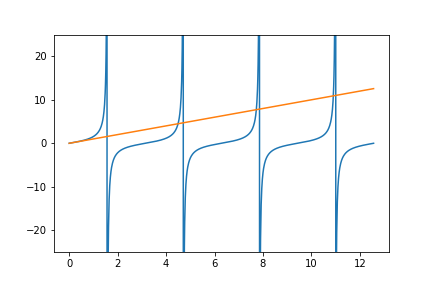
\includegraphics[width=4in]{tan.png}
\caption{tan(x) vs x}
\end{centering}
\end{figure}

The plots cross at infinitely many points. So, there are infinitely many solutions.
\item

\[\tan \lambda = \lambda \]

With usual techniques, we would get $\lambda$ near zero. But, we want solutions when $\lambda$ is very large. This is only possible when $\lambda \sim \frac{(2n+1)\pi}{2}$ where n is a very large integer.

We are going to assume
\[\lambda \sim \frac{\lambda_0}{\epsilon^\alpha}+ \lambda_1 \epsilon^\beta  \]
This is slightly different from the guess in the book.

Now, in this ansatz, as $\epsilon$ goes to zero, the second term disappears and the first term dominates.

\[ \frac{\lambda_0}{\epsilon^\alpha} \approx  \frac{(2n+1)\pi}{2} \]

\[\tan \bigg(\frac{\lambda_0}{\epsilon^\alpha}+ \lambda_1 \epsilon^\beta  \bigg) = \frac{\lambda_0}{\epsilon^\alpha}+ \lambda_1 \epsilon^\beta \]
\[ \tan \bigg(\frac{(2n+1)\pi}{2}+ \lambda_1 \epsilon^\beta  \bigg) =\frac{\lambda_0}{\epsilon^\alpha}+ \lambda_1 \epsilon^\beta \]

\[ \cot \bigg(- \lambda_1 \epsilon^\beta  \bigg) =\frac{\lambda_0}{\epsilon^\alpha}+ \lambda_1 \epsilon^\beta \]

\[-\frac{1}{\lambda_1 \epsilon^\beta }+ \frac{\lambda_1 \epsilon^\beta}{3}+ \hdots  =\frac{\lambda_0}{\epsilon^\alpha}+ \lambda_1 \epsilon^\beta \]

Doing dominant balance,
\[-\frac{1}{\lambda_1 \epsilon^\beta } \sim  \frac{\lambda_0}{\epsilon^\alpha}\]
\[\alpha = \beta \]
\[-\frac{1}{\lambda_1  }= \lambda_0 \]

Let $\alpha $ be 1.

\[ \frac{\lambda_0}{\epsilon} \approx  \frac{(2n+1)\pi}{2} \sim  \pi n\]
So,
\[n \sim \frac{1}{\epsilon} \]
and
\[\lambda_0 = \pi \]

Thus,
\[\lambda =  \frac{\pi}{\epsilon}-\frac{1}{\pi} \epsilon + o(\epsilon)\]


 \end{enumerate}
\end{enumerate}

\end{document}
